\documentclass{article}

% Geometry and layout
\usepackage[a4paper, total={7in, 10in}]{geometry}

% Math packages
\usepackage{amsmath, amssymb, amsthm, mathtools}
\usepackage{mathrsfs} 
\usepackage{bm} 
\usepackage[ruled,vlined,algo2e]{algorithm2e}

% Theorem environments
\newtheorem{theorem}{Theorem}
\newtheorem{proposition}{Proposition}
\newtheorem{lemma}{Lemma}
\newtheorem{corollary}{Corollary}
\newtheorem{definition}{Definition}
\newtheorem{example}{Example}
\newtheorem{remark}{Remark}

% References and Citations
\usepackage{hyperref}
\usepackage[capitalize,nameinlink]{cleveref}

% Lists and structuring
\usepackage{enumitem}

% Figures and Tables
\usepackage{graphicx, float}
\usepackage{caption, subcaption}
\usepackage{booktabs}

% Algorithms
\usepackage{algorithm}
\usepackage{algpseudocode}

% Colors for emphasis
\usepackage{xcolor}

% TikZ for diagrams
\usepackage{tikz}
\usetikzlibrary{arrows.meta, positioning, calc}

%fig shortcut
\newcommand{\fig}[2]{
    \begin{figure}
        \centering
        \includegraphics[width=\textwidth]{#1}
        \caption{#2}
        \label{fig:#1}
    \end{figure}
}

\title{Retrieval Augmented Generation}
\author{Elias W.J. Müller}
\date{FS26}

\begin{document}

\maketitle

\tableofcontents
\newpage
\section{RAG Introduction}
\paragraph{Motivation}

\begin{itemize}
    \item \textbf{Extrinsic LLM Hallucinations}: non factual to training data (wrong recall)
    \item \textbf{Intrinsic LLM Hallucinations}: non faithful to the input context, i.e., false retrieval from context (even if factual)
\end{itemize}

Many methods exist at different stages:
\begin{itemize}
    \item RAG (Inference): partial intrinsic hallucinations but primarily for extrinsic. But retrieval failures propagate or the model might ignore retrieved context.
    \item Instruction Tuning/ RLHF (Training): only for extrinsic hallucinations, but encourages fluency over faithfulness, and has no approach against source errors
    \item Contrastive Sampling (Training): Both intrinsic and extrinsic, but requires expensive hallucination labeled data
    \item HITL (Post-Generation): Both intrinsic and extrinsic, but not scalable and expensive
\end{itemize}



\section{Information Retrieval}
Distinction Sparse and Dense does not relate to data storage, but rather to the conceptual approach. \textit{Sparse} methods are the non-neural, statistical approaches (we count) whereas \textit{Dense} approaches rely on neural encoding methods incorporation sematic information. 
\subsection{Sparse Encoding}
Non-neural, statistical approaches that generally result in a sparse term-document representation in the query logic. To be used whenever speed and precision (in the metric sense) matters. But sparse encodings have a recall issue.
\subsubsection{Binary Indexing}
Trivial binary indication as \textit{vectorized} representations of queries in \textit{Term-Document} matrix $\in \mathbb{R}^{m\times n}$ (each term $\times$ each document section (e.g. chapter)), with $m$ terms (\textit{vocabulary} size) and $n$ documents (\textit{corpus} size). Indexing by creating a data structure that functions as a look-up-table for representing the terms we want to search over. \\
Generally, a RegEx approach that is \textit{fast and efficient} and \textit{re-executable} BUT:

\begin{itemize}
    \item \textbf{Very limited flexibility} in terms of expressiveness - only boolean queries (e.g. \texttt{AND, OR, NOT}): leverage vectors term for binary ops: $(1,0,0,1) \texttt{ AND }(1,1,0,0) \Rightarrow (1,0,0,0)$
    \item \textbf{High memory consumption} with extremely sparse representation in term-document matrix/ DB table \\ $(m \times n) / 8 \text{ bits} = \text{ bytes}$
    \item \textbf{Limited representativeness}: no relevance ranking since all terms are equally important
\end{itemize}

\subsubsection{Term-Frequency Inverse Document-Frequency (TF-IDF)}
A Bag-of-Words (BoW) approach representing the term-document matrix with number of appearances in the corpus. Based on the probabilistic idea that term appearances make documents prototypical. \\

High TF-IDF weights are thus assigned to a term $t$ if it appears only in a few documents in the corpus but in these with high frequency (discriminative), and low weights if $t$ appears in most/all documents and is thus not discriminative.\\

\noindent\textbf{TF-IDF} combines TF and IDF we get: $\text{TF-IDF}_{t,d}= \text{TF}_{t,d} \times \text{IDF}_{t}$

\begin{itemize}
    \item \textbf{Term Frequency} term counts normalized by the number of terms in the documents after \textit{stop-word} removal: 
    $$
    \text{tf}_{t,d}=\frac{f_{t,d}}{\Sigma_{t'\in d}f_{t',d}}
    $$
    Isomorphic approach, i.e. BoW ignores word order of the term appearances. Essentially, we get high weights for words that appear frequently.
    \item \textbf{Inverse Document Frequency} assigns different weights to different words, giving \textit{low weight to common less indicative words} and \textit{high weights to rare and more indicative words} in terms of the corpus at hand.
    \begin{align*}
        \text{Document Frequency (by term weight for document appearance):}\qquad \text{df}_t &=\sum_{d\in \mathbb{D}} 1, \text{ if } t \in d \\
        \textbf{Inverse Document Frequency:} \qquad \text{idf}_t &= \log \frac{\Sigma_{d\in \mathbb{D}}1}{\text{df}_t}, \text{ if } t \in d
    \end{align*}
    We use the IDF for computational efficiency, since df-values can be very large for large corpora.\\
    Since the vocabulary $V$ is compiled from the corpus $\mathbb{D}$ we can only represent tokens in $V$. With $n$ documents 
    $$1 \leq \text{df}_t \leq n \implies 1 \leq \frac{n}{\text{df}_t} \leq n \implies 0 \leq \text{idf}_t \leq \log n$$
    However, idf can only be $0$ for Query-Terms that are Out-Of-Domain and not for tokens is $V$. 
\end{itemize}

\noindent\textbf{Drawbacks of TF-IDF:}
\begin{itemize}
    \item \textbf{Linear Scaling:} TF grows linearly with raw count, but importance has diminishing returns --- going from 1$\to$2 occurrences is more meaningful than 99$\to$100. TF-IDF has no saturation mechanism and thus over-rewards high-frequency terms
    \item \textbf{Varying document lengths:} longer documents have higher TF due to more words, not higher relevance
    \item \textbf{Rigid:} static formula with no adjustable parameters $\rightarrow$ cannot adapt to specific corpora or tasks
    \item \textbf{Count-based:} does not utilize prior knowledge about the corpus --- essentially fancy RegEx
\end{itemize}

\subsubsection{BM25}
BM25 (Best Matching 25) augments TF-IDF with advanced frequency terms, document lenght normalization and prevention of extremes, to rank documents by their probability of relevance (\textit{Probability Ranking Principle}). Its the SOTA Benchmark as a tunable and controllable approach:
$$
\text{BM25}_{q,d} = \sum_{i=1}^{n} \text{IDF}(q_i) \cdot \frac{f_{q_i,d} \cdot (k_1 + 1)}{f_{q_i,d} + k_1 \cdot \left(1 - b + b \cdot \frac{|d|}{\text{avg. dl}}\right)}
$$
where $f_{q_i,d}$ is the term frequency of $q_i$ in $d$, $|d|$ the document length, $k_1$ a TF saturation parameter, $b$ a length normalization parameter, and
$$
\text{IDF}(q_i) = \log\left(\frac{N - n(q_i) + 0.5}{n(q_i) + 0.5} + 1\right)
$$
with $N$ the corpus size, $n(q_i)$ the number of documents containing $q_i$, and $0.5$ a smoothing term to avoid $\text{df}_t = 0$ for query terms absent from the corpus. This also make its less sensitive to term frequencies, thus resulting in a less pronounced linear scaling effect (more saturation).\\

\textit{Memory and Storage Challenges} are, however, a common issue with BM25 thus we required an \textit{Inverted Index} for large scale corpora settings.

\subsubsection{Inverted Index}
The mapping $f:d\mapsto t$ is reversed, s.t., $g:t\mapsto d$. Wrt. the TD-Matrix this means that we no longer consider the Term-Document mapping, but store $\texttt{Term|TF}\mapsto\texttt{Inverted Linked List} \text{ (Chain of Document IDs)} \rightarrow$ No more zeros and space-efficient storage via data structs like \texttt{json}

\subsubsection{BM25 ranking with Inverted Index}
Given $\mathcal{D}$ documents and query $\mathcal{Q}=\{q_1, \dots, q_n\}$ we return a ranked list of top $k$ documents.\\

\begin{algorithm}[ht]
\caption{BM25 Ranking: Ranking and Returning Results}
\label{alg:bm25}
\KwIn{Documents $\mathcal{D}$, query $\mathcal{Q}=\{q_1,\dots,q_n\}$, params $k_1, b$, cutoff $k$}
\KwOut{Ranked list of the top $k$ documents}

\textbf{Initialize:} empty inverted index $I$, empty list of doc lengths $L$, doc count $N$\;
\BlankLine

\textbf{Step 1: Build Inverted Index}\;
\ForEach{document $D_i$}{
    Split $D_i$ into terms $\{t_1, t_2, \dots\}$\;
    Compute term frequencies for $D_i$\;
    Update $I[t]$ with $(D_i, \mathrm{tf})$ for each term $t$\;
    Compute length $L[D_i] = \mathrm{len}(D_i)$\;
}
Compute average document length $\mathrm{avg.dl} = \dfrac{\sum L[D_i]}{N}$\tcp*{normalize}
\BlankLine

\textbf{Step 2: Compute BM25 Scores}\tcp*{init empty dictionary $\mathit{scores}$}
\ForEach{term $q \in \mathcal{Q}$}{
    \If{$q \in I$}{
        $\mathrm{idf}(q) \gets \log\!\left(\dfrac{N - |I[q]| + 0.5}{|I[q]| + 0.5}\right)$\;
        
        \ForEach{$(D_i, \mathrm{tf}) \in I[q]$}{
            $L_d \gets L[D_i]$\;
            
            $\mathit{score} \gets \mathrm{idf}(q) \cdot
                \dfrac{\mathrm{tf}\cdot(k_1+1)}
                      {\mathrm{tf} + k_1 \cdot \left(1 - b + b \cdot \frac{L_d}{\mathrm{avg.dl}}\right)}$\;
                      
            $\mathit{scores}[D_i] \gets \mathit{scores}[D_i] + \mathit{score}$\;
        }
    }
}
\BlankLine

\textbf{Step 3: Rank Documents}\;
Sort $\mathit{scores}$ in descending order\;
\Return top $k$ documents with the highest scores\;
\end{algorithm}
 

\subsection{Dense Retrieval}
\subsubsection{Dense Encoding: Vector Space Model}
\textbf{Motivation:} While sparse encodings are easy and interpretable, the do not model the semantics.\\

\textbf{Trivial} approach: use the TF-vectorized document representations (documents x term (count) matrix) and use some similarity metric: 
\begin{itemize}
    \item Vector Difference $e_{d_1}- e_{d_2}$: very easy but sensitive to absolute differences in TF and not normalized wrt. doc length (longer docs have more diversity naturally)
    \item \textbf{Cosine Similarity}
    $$
    \text{sim}(e_{x_1}, e_{x_2})= \frac{e_{x_1}\cdot e_{x_2}}{\Vert e_{x_1} \Vert \Vert e_{x_2} \Vert}
    $$

    we could apply this to some $e_{d_1}, e_{d_2}$, but we want to find relevant documents with a \textbf{query}: $\text{sim}(e_{q}, e_{d})$. The inner product, however, cannot be computed given $e_q \in \mathbb{R}^{1 \times m}$ (TF-IDF row) and $e_d \in \mathbb{R}^{n \times 1}$ (TF-IDF col)\\

    $\rightarrow$ \textit{embed query and document in the same dimensionality} using Word Embeddings (Word2Vec) and representing $e_q, e_d$ as the average of their word embeddings. (doc embeddings can be precomputed and stored in RAM for efficiency)
\end{itemize}

\subsubsection{Dense Encoding: Nearest Neighbor Search}
How to apply the Cosine Similarity.
\paragraph{Nearest Neighbor Search}
\textit{Brute-Force/ exhaustive} computation of all similarities: $\arg \max \text{sim}_{d_i \in D}(e_q,e_{d_i})$ in $\mathcal{O}(n)$ for one query $\mathcal{O}(m\cdot n)$ for $m$ queries. Operations with complexity $n \cdot k$ since inner product.
$$
\text{Matrix-based Comp/ Score Matrix:} \quad S=\frac{M_QM_D}{\Vert M_Q\Vert_2 \Vert M_D \Vert_2} \quad S_{i,j}\in [-1,1],
$$

\paragraph{Approximate Nearest Neighbor Search}
Given set of documents $D$, a text encoder $e$ s.t. each output $\mathbb{R}^k$, find documents $D^* \subseteq D$ s.t. (with tolerance $\epsilon$):
$$
\forall d_i^* \in D^* \implies \text{dist}(e_q, e_{d^*_i})\leq (1+ \epsilon) \cdot \min_{d \in D} \text{dist}(e_q, e_d)
$$

dist$(\cdot)$ can be any monotonic function:
\begin{itemize}
    \item \textbf{Euclidean Distance ($L_2$):} $\text{dist}(e_{\mathbf{q}}, e_{\mathbf{d}}) = \sqrt{\sum_{i=1}^{k} \left(e_{q_i} - e_{d_i}\right)^2}$ - straight-line distance; sensitive to magnitude
    \item \textbf{Cosine Distance:} $\text{dist}(e_{\mathbf{q}}, e_{\mathbf{d}}) = 1 - \dfrac{e_{\mathbf{q}} \cdot e_{\mathbf{d}}}{\|e_{\mathbf{q}}\|_2 \, \|e_{\mathbf{d}}\|_2}$ - angle-based, magnitude-invariant; standard for embeddings
    \item \textbf{Manhattan Distance ($L_1$):} $\text{dist}(e_{\mathbf{q}}, e_{\mathbf{d}}) = \sum_{i=1}^{k} |e_{q_i} - e_{d_i}|$ - more robust to outliers than $L_2$
    \item \textbf{Jaccard Distance:} $\text{dist}(b_{\mathbf{q}}, b_{\mathbf{d}}) = 1 - \dfrac{|b_{\mathbf{q}} \cap b_{\mathbf{d}}|}{|b_{\mathbf{q}} \cup b_{\mathbf{d}}|}$ - set overlap (intersection over union); for binary/sparse
\end{itemize}

Options for Approximate NNS
\begin{itemize}
    \item \textit{Model Quantization} to reduce space complexity with some performance degradation. (e.g. \verb|fp32| $\rightarrow$ \verb|int8|)
    \item \textit{Matrix Factorization}: SVD or Canonical Correlation Analysis
    \item \textit{Clustering-Based Approaches}: $k$-means or hierarchical clustering
    \item \textit{Hashing-Based Approaches}: Locality-Sensitive Hashing (LSH)
\end{itemize}

\subsubsection{Dense Encoding: Locality-Sensitive Hashing}
We use Local Sensitivity (Bucketing) for approximate NNS. Given tow doc embeddings, some similarity measure, a threshold $s$ and a hash function $h$, then we can hash similar docs into the same bucket and only search within this:
\begin{itemize}
    \item sim$(e_{d_1}, e_{d_2}\geq s) \rightarrow h(e_{d_1})=h(e_{d_2})$
    \item sim$(e_{d_1}, e_{d_2}< s) \rightarrow h(e_{d_1})\neq h(e_{d_2})$
\end{itemize}

\paragraph{Sampling Strategy}
\begin{enumerate}
    \item \textbf{Sampling Strategy}: Choose set of hash functions (e.g. Bit Sampling, i.e. given binary repr, a bit sampling $h$ selects $n$ indices: $h_1 = [1,3,4] \rightarrow h_1((1,0,0,1,1,0))= 011$). \\

    For $n$-bit sampling you can have $2^n$ hash functions.

    \item \textbf{ Create Hash Table}: Apply the selected hashing functions to all documents and create the buckets (hash-values $\times$ hash-functions)

    \item \textbf{NN search within}: Apply hash function to the vectorized repr of the query (e.g. binary if bit-sampling), and perfrom NN-search in each bucket that was matched by the hash function on the query: 
    $$
    \verb|return| \arg \max_{d_i \in [d_3, d_6]}\text{sim}(e_q,e_{d_i}) \qquad \text{for each matched bucket per hash function}
    $$

    \item \textit{Hyperparam selection} ($K$ hash functions, $L$ buckets):
    \begin{itemize}
        \item \textbf{Larger $K$ (stricter hashing):} smaller buckets $\to$ fewer NN candidates, but more false negatives $\to$ lower Recall. Pick $K$ so bucket size stays manageable.
        \item \textbf{Larger $L$ (more redundancy):} more hash tables tables required $\to$ higher chance a true neighbor collides somewhere $\to$ fewer false negatives, higher Recall. Cost: repeated NN computation across tables + more memory to store the extra hash tables.
    \end{itemize}
\end{enumerate}

\subsubsection{Dense Retrieval Learned Embeddings: Optimization Objectives}
The choice of embeddings matters a lot in training a model. While cosine similarity is common, recent research has uncovered limitations.

\paragraph{(1) Cosine similarity is not automatically meaningful (Steck et al.\ 2024).}
\begin{itemize}
    \item Similarity scores are an \emph{artifact of regularization}, not an intrinsic property of the embeddings:
    \begin{itemize}
        \item \textbf{Drop-out style:} penalizes the \emph{product} of embedding matrices \emph{jointly} $\to$ arbitrary / meaningless cosine scores.
        \item \textbf{Weight-decay style:} penalizes each matrix \emph{separately} $\to$ well-defined cosine scores.
    \end{itemize}
    \item Modern models mix both (both are $L_2$ reg.) $\Rightarrow$ explains why cosine \emph{sometimes} works, sometimes not.
    \item \emph{Intuition:} reg.\ can \emph{anisotropically} stretch/squeeze the space, so cosine ends up measuring \emph{geometric distortion}, not semantics $\Rightarrow$ bad retriever $\Rightarrow$ ``RAG fails because the retriever is bad''.
    \item \emph{Takeaway:} the \textbf{training objective}, not the metric, decides whether geometry is semantically meaningful.
\end{itemize}

\paragraph{(2) What we want $\approx$ a margin objective (SVM analogy).}
\begin{itemize}
    \item Pull query \emph{close} to relevant docs, push \emph{far} from irrelevant ones.
    \item Same shape as soft-margin SVM: $\min_{\mathbf{w},b}\ \tfrac{1}{2}\mathbf{w}^T\mathbf{w} + C\sum_{i=1}^{N}\max\{0,\,1-y_i(\mathbf{w}_i^T\mathbf{x}_i+b)\}$, $y_i\in\{-1,1\}$.
    \item \emph{Mapping:} separating hyperplane $\leftrightarrow$ relevant/irrelevant boundary; margin $\leftrightarrow$ how confidently pos beats neg; support vectors $\leftrightarrow$ hard (near-boundary) negatives.
\end{itemize}

\paragraph{(3) Concrete training objectives (contrastive losses).}
Setup: query $\mathbf{q}$, positive doc $\mathbf{d}^+$, negative doc $\mathbf{d}^-$.
\begin{itemize}
    \item \textbf{Margin / triplet hinge} -- \emph{pairwise}:
    $$\mathcal{L}_\theta = \sum_{\mathbf{d}^+\in D^+}\sum_{\mathbf{d}^-\in D^-}\max\!\big(0,\ \mathrm{sim}(\mathbf{q},\mathbf{d}^+)-\mathrm{sim}(\mathbf{q},\mathbf{d}^-)+\epsilon\big)$$
    $\epsilon$ = margin (required gap; controls sensitivity). \emph{Note on signs:} as written this treats $\mathrm{sim}$ as a \emph{distance} (want $\mathrm{sim}(q,d^+)$ small). For a true similarity (higher = better) the standard form flips to $\max(0,\,\epsilon-\mathrm{sim}(q,d^+)+\mathrm{sim}(q,d^-))$.
    \item \textbf{InfoNCE / softmax NLL}-- \emph{1 pos vs.\ $n$ negs}:
    $$\mathcal{L}_\theta = -\log\frac{e^{\mathrm{sim}(\mathbf{q}_i,\mathbf{p}_i^+)}}{e^{\mathrm{sim}(\mathbf{q}_i,\mathbf{p}_i^+)}+\sum_{j=1}^{n}e^{\mathrm{sim}(\mathbf{q}_i,\mathbf{p}_j^-)}}$$
    \emph{Intuition:} cross-entropy that wants the positive to ``win'' the softmax over all negatives. More negatives $\to$ harder, better-calibrated gradient.
    \item \textbf{Temperature-scaled InfoNCE}:
    $$\mathcal{L}_\theta = -\log\frac{e^{\mathrm{sim}(\mathbf{q}_i,\mathbf{p}_i^+)/\tau}}{e^{\mathrm{sim}(\mathbf{q}_i,\mathbf{p}_i^+)/\tau}+\sum_{j=1}^{n}e^{\mathrm{sim}(\mathbf{q}_i,\mathbf{p}_j^-)/\tau}}$$
    $\tau$ = temperature. \emph{Intuition:} small $\tau$ $\to$ sharp softmax, focuses gradient on the \emph{hardest} negatives; large $\tau$ $\to$ softer, treats negatives more uniformly.
\end{itemize}

\paragraph{(4) Qwen3-Embedding: a concrete modern recipe.}
\textbf{Loss = ``souped-up'' InfoNCE.} Same InfoNCE skeleton as before, but the denominator $Z_i$ pools \emph{five} sources of negatives, each gated by a mask $m$:
$$\mathcal{L}_{\text{embedding}} = -\frac{1}{N}\sum_{i}^{N}\log\frac{e^{s(q_i,d_i^+)/\tau}}{Z_i}$$
$$Z_i = \underbrace{e^{s(q_i,d_i^+)/\tau}}_{\text{(1) positive}} + \underbrace{\sum_k^K m_{ik}e^{s(q_i,d_{i,k}^-)/\tau}}_{\text{(2) }K\text{ hard negs}} + \underbrace{\sum_{j\neq i} m_{ij}e^{s(q_i,q_j)/\tau}}_{\text{(3) in-batch }q\text{--}q} + \underbrace{\sum_{j\neq i} m_{ij}e^{s(d_i^+,d_j)/\tau}}_{\text{(4) in-batch }d\text{--}d} + \underbrace{\sum_{j\neq i} m_{ij}e^{s(q_i,d_j)/\tau}}_{\text{(5) in-batch }q\text{--}d}$$
\begin{itemize}
    \item \textbf{Hard negatives} $d_{i,k}^-$: mined to be lexically similar (e.g.\ high BM25) but semantically wrong $\Rightarrow$ forces fine-grained discrimination, not just easy random rejects.
    \item \textbf{In-batch negatives} (3)--(5): reuse every other example in the batch ``for free'' as negatives across all pairings ($q$--$q$, $d$--$d$, $q$--$d$) $\Rightarrow$ huge effective negative count at ~no extra cost.
    \item \textbf{Mask factor $m$ = false-negative guard} (the key ``improvement''):
    $$m_{ij} = \begin{cases} 0, & \text{if } s_{ij} > s(q_i,d_i^+) + 0.1 \ \text{ or } \ d_j = d_i^+ \\ 1, & \text{otherwise} \end{cases}$$
    \emph{Intuition:} an in-batch ``negative'' that scores \emph{higher} than the true positive (by $>0.1$) is almost certainly a duplicate / mislabeled positive $\Rightarrow$ zero it out so the loss never penalizes a correct match. Prevents positive leakage from batch construction.
\end{itemize}

\begin{figure}[H]
    \centering
    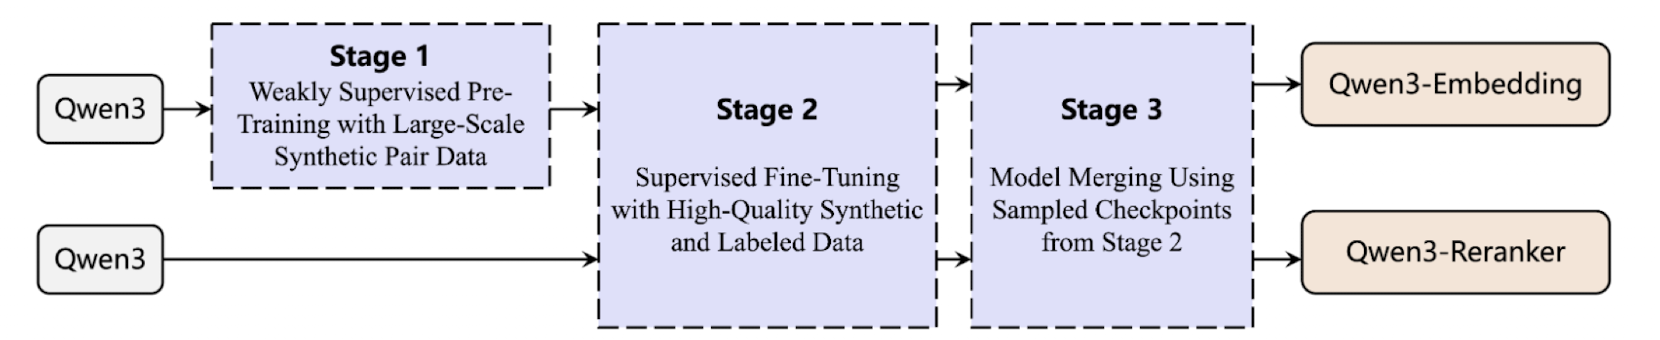
\includegraphics[width=0.8\linewidth]{img/Owen3Emb.png}
    \caption{Qwen3-Embedding}
    \label{fig:Owen3Emb}
\end{figure}

\subsubsection{Dense Retrieval Learned Embeddings: Document Sampling Strategies}
Given query $\mathbf{q}$ and positive $\mathbf{d}^+$, how to pick negatives from $D$? Five strategies on a \emph{cheap/weak $\to$ expensive/informative} spectrum:

\begin{enumerate}
    \item \textbf{Random:} $\mathbf{d}^- \sim D\setminus\{\mathbf{d}^+\}$ — cheap, but mostly trivial negatives + false-negative risk.
    \item \textbf{In-Batch:} other queries' positives in batch $\mathcal{B}$ as negatives — free, but quality depends on batch composition.
    \item \textbf{Cross-Batch:} negatives from outside $\mathcal{B}$ (memory queue) — more diverse, but needs extra memory.
    \item \textbf{Hard Negative:} $\text{top}_k$ by $\text{sim}(\mathbf{q},\mathbf{d})>\tau$ — similar-but-wrong docs give strong gradient, but expensive + overfitting + \emph{highest} false-negative risk.
    \item \textbf{Semantic-Aware:} negatives sharing prior-knowledge features $\phi(\mathbf{d})=\phi(\mathbf{d}^+)$ — context-relevant, but needs metadata $\phi$.
\end{enumerate}

\noindent\textbf{Key threads:} (i) \emph{false negatives} plague 1, 2, 4 (worst for hard negatives, since top-similar docs are often unlabeled positives) — this is exactly what Qwen3's mask $m_{ij}$ fixes. (ii) Strategy 4 = \emph{dynamic} hardness (model-scored, drifts, re-mine), Strategy 5 = \emph{static} hardness (fixed features). (iii) $\tau$ here is a \emph{similarity threshold}, not the softmax temperature.

\subsection{Information Retrieval Evaluation}
\textbf{Expectation:} a good retriever must have \textit{high recall and precision, fast response, and robust query understanding} (handle varying complexity, formulations and ambiguities)

\begin{itemize}
    \item \textbf{Precision:} $tp/(tp+fp)$ (Precision@k) - ignores order of retrieval
    \item \textbf{Recall:} $tp/(tp+fn)$ (Recall@k) - ignores order of retrieval
    \item \textbf{Accuracy:} $(tp+tn)/n$ - not used, since we often don't care about irrelevance identification performance, and imbalanced datasets (most irrelevant)
    
    \item \textbf{Mean Reciprocal Rank:} order/ rank of relevant retrieval (0.5 if at second position since $1/2$). The mean simply averages over a set of queries in an IR test set
    $$
    MRR = \frac{1}{n}\sum^n_{i=1}RR(q_i) \qquad \text{with}\qquad RR(q) = \frac{1}{\text{rank of the first relevant retireval}}
    $$
    While MRR is \textit{indicative} (the higher the better) and \textit{interpretable}, it is biased since only \textit{the first relevant matters}, and it is \textit{narrow} (only suitable if only one relevant document per query). Importantly, it has no explanation of the relative \textit{ranking quality} (if multiple relevant docs exist) - the most relevant can be very low
    
    \item \textbf{Normalized Discounted Cumulative Gain NDCG@k:} compares ranking of \textit{relevance scores} to ideal GR ranking with cut-off $k$:
    $$
    \text{NDCG@k} = \frac{\text{DCG@k}}{\text{IDCG@k}} \qquad \text{where} \quad \text{DCG@k}=\sum^k_{i=1}\frac{\text{rel}_i}{\log_2(i+1)}\
    $$

    $rel_i$ being some relevance score (cosine sim. or binary) and DCG@k: discounted CG with IR ranking and IDCG@k: ideal discounted CG with GT ranking. Note $\text{CG@k}=\sum^k_{i=1}\text{rel}_i$ but we use DCG since logarithmic discout assigns lower gain when relevant items appear further down (difference 1 to 2 is larger than difference 2 to 3). \\

    \textit{Pros:} rank aware, variable relevance scores, and normalized\\
    \textit{Cons:} relevance score selection dependent, requires GT (not stand-alone eval metric)

    \item \textbf{Miscellaneous} (online/behavioral metrics, log-based, no GT relevance labels needed):
    \begin{itemize}
        \item \textbf{Click-Through Rate (CTR):} $\text{Clicks}/\text{Impressions}$ - ratio of users who click vs. those who only see it
        \item \textbf{Session Success Rate (SSR):} $\text{Successful Sessions}/\text{Total Sessions}$ - ratio of sessions where the user achieves their goal (e.g.\ click, find answer)
        \item \textbf{Zero Result Rate (ZRR):} $\text{Zero Result Queries}/\text{Total Queries}$ - ratio of queries returning no results
    \end{itemize}
\end{itemize}


\section{Language Modeling}
\subsection{LLM Basics}
Probabilistic natural language modeling form a sequence of $n$ tokens $X=(x_1,\dots, x_n)$ given a vocabulary $V$, basing on the causality of languages and their context dependence (requirement): 
$$
P(X)= \prod_{i=1}^nP(x_i|x_1, \dots , x_{i-1})
$$

\textbf{Ngram LM} based on the \textit{Markov Assumption} (generated token counts as well): $P(X)=\prod_{i=1}^nP(x_i|x_{i-N+1:i-1}) \rightarrow \text{e.g. Bigram} P(X)=\prod_{i=1}^nP(x_i|x_{i-1})$. \\

This prediction is based on the surroundings of the generated tokens by extracting a \textit{probability distribution} given the corpus.

\subsubsection{Count-Based LM}
Count how many times a target work appears in different contexts (\texttt{C(target|context$_i$)}). Goal is to find some \texttt{C(target|context$_j$)} $\gg$ \texttt{C(target|context$_i$)}: \textit{Maximum Likelihood Estimation (MLE)}:
$$
P_{MLE}(\text{target} \vert \text{context})=\frac{C(\text{context,target})}{\sum_{x\in V}C(\text{context,x)}}
$$

This can be applied to ngram LM: 

$$
P_{MLE}(x_i \mid x_{i-N+1:i-1}) = \frac{C(x_{i-N+1}, \dots, x_i)}{C(x_{i-N+1}, \dots, x_{i-1})} \qquad \text{Bigram:}\quad  P_{MLE}(x_i \mid x_{i-1}) = \frac{C(x_{i-1}, x_i)}{\sum_{x \in V} C(x_{i-1}, x)} = \frac{C(x_{i-1}, x_i)}{C(x_{i-1})}
$$

Since we only approximate the true probability all models are \textit{potentially wrong}, and when $N$ gets large, the counts become very sparse. thus we logarithmize the probabilities to avoid underflow: $P_1 \times P_2 \times P_3 = \exp(\log P_1 + \log P_2 +\log P_3)$

\textbf{Issue:} Many Ngrams will never occur in the corpus, thus $P(X)=0$. We can apply 

\paragraph{Smoothing.} Reserve probability mass for unseen ngrams by treating rare events as if seen more often (\textit{add artificial counts}), while preserving $\sum_i p_i = 1$:
\begin{itemize}
  \item \textit{Laplace (add-1):} $P(x_i \mid x_{i-1}) = \frac{C(x_{i-1},x_i)+1}{C(x_{i-1})+|V|}$ --- add 1 to every count; over-smooths when $|V|$ is large.
  \item \textit{Add-$k$:} $P(x_i \mid x_{i-1}) = \frac{C(x_{i-1},x_i)+k}{C(x_{i-1})+k|V|}$ --- tunable $k<1$ softens the over-smoothing.
  \item \textit{Kneser-Ney:} discount each seen count by a fixed $\delta$ and back off to a lower order, 
  $$P_{KN}(x_i \mid x_{i-1}) = \frac{\max(C(x_{i-1},x_i)-\delta,\,0)}{\sum_{x\in V}C(x_{i-1},x)} + \lambda_{x_{i-1}}\,P_{KN}(x_i)$$
  , where the lower-order term is a \textit{continuation probability} (how many distinct contexts $x_i$ follows), not the raw unigram.
\end{itemize}

\paragraph{Interpolation \& backoff.} The zero-count problem ultimately stems from contexts being too long. Rather than trusting a single ngram order, mix all orders:
$$
\hat{P}(x_i \mid x_{i-2}, x_{i-1}) = \lambda_1 P(x_i) + \lambda_2 P(x_i \mid x_{i-1}) + \lambda_3 P(x_i \mid x_{i-2}, x_{i-1}), \qquad \sum\nolimits_* \lambda_* = 1,
$$
with the $\lambda$s estimated on held-out data via \textbf{Expectation Maximization}. In short: \textit{smoothing} redistributes mass \emph{within} a fixed context, \textit{interpolation} mixes \emph{across} context lengths --- Kneser-Ney does both.\\

\textbf{Cons.}
\begin{itemize}
    \item Bad probability estimation: very large corpora required
    \item Curse of dimensionality: memory intense to store counts
    \item Limited Context length: Markov assumption
    \item Smoothing dependency: we always shift some
\end{itemize}

\subsubsection{Auto-regressive LM}
Using high dimensional encodings (word embeddings) to model probabilities.

\subsubsection{LM Performance Evaluation}

\subsection{LLM Paradigms}
\section{RAG Engineering}
\subsection{Backend Engineering}
\subsection{Frontend Engineering}
\subsection{System Testing}
\subsection{RAG Applications}
\section{MISC}
\subsection{Guest Lectures}


\end{document}